\section{Moderne Symmetrische Chiffren}

\subsection{Lineare Abbildungen}


\subsection{Feistel-Cipher}
\subsubsection{}
$F: \{0, 1\}^4 \times \{0, 1\}^4 \to \{0, 1\}^4 $ mit $F(X, Y) = X \xor Y$\\
die Rundenzahl $n = 2$,\\
der Plaintext $ P = 10011100$ und\\
die Rundenschlüssel $K_1 = 0101 $und $K_2 = 1100$.
\paragraph{Berechnen Sie den Ciphertext $C$.}

\begin{align}
 L_i &= R_{i-1}\\
 R_i &= L_{i−1} \xor F(R_{i−1}, K_i)
\end{align}

\begin{tabular}{cc|ll}
Rnd & $K_i$ & $L_i$  & $R_i$    \\ \hline
0   & ---   & 1001 & 1100  \\
1   & 0101  & 1100 & 0000  \\
2   & 1100  & 0000 & 0000  
\end{tabular}

\paragraph{Berechnen Sie aus $C$ wieder den Plaintext $P$}.


\begin{align}
 R_{i} &= L_{i+1}  \\
 L_{i} &= R_{i+1} \xor F(R_{i},K_{i+1})
\end{align}

\begin{tabular}{cc|ll}
Rnd & $K_i$ & $L_i$  & $R_i$    \\ \hline
2   & 1100  & 0000 & 0000 \\
1   & 0101  & 1100 & 0000 \\
0   & ---   & 1001 & 1100  
\end{tabular}


\subsubsection{}
Eine Feistel-Funktion ist definiert durch $F(X, Y) = X$. Berechnen Sie den Ciphertext
$C$ in Abhängigkeit von einer beliebigen Rundenzahl $n$ und dem Plaintext $P = (L_0, R_0)$
Wie gut ist die dadurch erreichte Verschlüsselung?

\begin{tabular}{cc|>{$}c<{$}>{$}c<{$}}
Rnd & $K_i$ & L_i  & R_i    \\ \hline
0   & ---   & a        & b         \\
1   & ---   & b        & b \xor a  \\
2   & ---   & b \xor a & a         \\  
3   & ---   & a        & b         \\  
\end{tabular}

\begin{equation}
f(n, (a,b) ) = %
	\begin{cases}
	(a,b)        ,& n \mod 3 = 0 \\
	(b,b \xor a) ,& n \mod 3 = 1 \\
	(b \xor a,a) ,& n \mod 3 = 2 
	\end{cases}
\end{equation}


\subsection{DES-Details}
\subsubsection{Zeigen Sie, dass die DES-Expansionspermutation eine lineare Abbildung ist.}

\begin{equation}
A = \begin{array}{*{14}{r}}
(& 31 &  0 &  1 &  2 &  3 &  4 &  3 &  4 &  5 &  6 &  7 &  8 & \\
 &  7 &  8 &  9 & 10 & 11 & 12 & 11 & 12 & 13 & 14 & 15 & 16 & \\
 & 15 & 16 & 17 & 18 & 19 & 20 & 19 & 20 & 21 & 22 & 23 & 24 & \\
 & 23 & 24 & 25 & 26 & 27 & 28 & 27 & 28 & 29 & 30 & 31 &  0 &)
\end{array}
\qquad 
\end{equation}
Sei $P \in \mathbb{N}^{32 \times 48}$ die entsprechende Permutationsmatrix für $A$ 
und $f:\, A^{32} \to A^{48} ,\quad x \mapsto P \cdot x$ die Permutationsfunktion.

\textbf{zZ: f ist linear}\\

Sei $ x,y \in A^{32} $ mit $ x = (x_0, x_1, \ldots, x_{31} )$ und 
 $ y = (y_0, y_1, \ldots, y_{31} )$ 
 dann ist

\begin{align}
f(\alpha x) &=  \begin{array}{*{14}{r}}
(&\alpha x_{31} &  \alpha x_{0} &  \cdots &  \alpha x_{8} \\
 &\alpha x_{7}  &  \alpha x_{8} &  \cdots & \alpha x_{16} \\
 &\alpha x_{15} &  \alpha x_{16} & \ddots & \vdots        \\
 &\alpha x_{23} &  \alpha x_{24} & \cdots & \alpha x_{0}  &)\\
\end{array} \\
& = \alpha  \begin{array}{*{12}{r}}
 &(x_{31} &  x_{0} &  \cdots &  x_{8} \\
 & x_{7}  &   x_{8} &  \cdots &  x_{16} \\
 &x_{15} &   x_{16} & \ddots & \vdots        \\
 &x_{23} &   x_{24} & \cdots &  x_{0} &) \\
\end{array}\\
&= \alpha f(x)
\end{align}

\begin{align}
f(x+y) &=  \begin{array}{*{14}{r}}
(& x_{31} + y_{31} &  x_{0}  +y_{0}  &  \cdots &  x_{8} + y_{8}\\
 & x_{7}  + x_{7}  &  x_{8}  +y_{8}  &  \cdots & x_{16} + y_{16} \\
 & x_{15} + y_{15} &  x_{16} +y_{16} &  \ddots & \vdots        \\
 & x_{23} + y_{23} &  x_{24} +y_{24} &  \cdots & x_{0} +y_{0} &)
\end{array} \\
 & = \begin{array}{*{12}{r}}
 &(x_{31} &  x_{0} &  \cdots &  x_{8} \\
 & x_{7}  &   x_{8} &  \cdots &  x_{16} \\
 &x_{15} &   x_{16} & \ddots & \vdots        \\
 &x_{23} &   x_{24} & \cdots &  x_{0} &) \\
\end{array} + 
\begin{array}{*{12}{r}}
 &(y_{31} &  y_{0} &  \cdots & y_{8} \\
 & y_{7}  &   y_{8} &  \cdots &  y_{16} \\
 &y_{15} &   y_{16} & \ddots & \vdots        \\
 &y_{23} &   y_{24} & \cdots &  y_{0} &) \\
\end{array}\\
&= f(x)+f(y)
\end{align}
\qed

\subsubsection{Zeigen Sie, dass die DES S-Boxen keine lineare Abbildung sind.}

\textbf{zZ. $S_i$ ist nicht linear.} 
Wir nehmen die S1-Box und sei $x = 0 \wedge \alpha = 2$ 

\begin{align}
 \operatorname*{S1}(\alpha x) &=  \operatorname*{S1}(000000_2)      \\
				              &= 1110_2  = 14_{10}                  
\end{align}
\begin{align}
  \alpha  \operatorname*{S1}(x) &= 2 \operatorname*{S1}(000000_2)  \\
				 &= 2_{10} * 1110_2 = 28_{10}
\end{align}
\begin{equation}
\Rightarrow 	\operatorname*{S1}(\alpha x) \ne \alpha \operatorname*{S1}(x)			
\end{equation}
\qed

\subsubsection{Geben Sie für die DES-Permutation die Zykelschreibweise an.}
\begin{equation}
A = \left (\begin{array}{*{32}{r}}
0&1&2&3&4&5&6&7&8&9&10&11&12&13&14&15&16&17&18&19&20&21&22&23&24&25&26&27&28&29&30&31	\\
15&6&19&20&28&11&27&16&0&14&22&25&4&17&30&9&1&7&23&13&31&26&2&8&18&12&29&5&21&10&3&24
\end{array}\right )
\end{equation}
	
\begin{equation}
\text{Zyklen:}  
(0\,15\,9\,14\,30\,3\,20\,31\,24\,18\,23\,8)
(1\,6\,27\,5\,11\,25\,12\,4\,28\,21\,26\,29\,10\,22\,2\,19\,13\,17\,7\,16)
\end{equation}												

\subsubsection{Zeigen Sie, dass für den DES Schlüssel $K = 0xE0E0E0E0F1F1F1F1$
(inklusive Parity-Bits) alle Rundenschlüssel identisch sind. Warum gilt in
diesem Fall $DES(K, DES(K, M)) = M$ (d.h. Ver- und Entschlüsselung sind
identisch)?}

\begin{equation}
K=\begin{matrix}
1 & 1 & 1 & 0 & 0 & 0 & 0 & 0 \\
1 & 1 & 1 & 0 & 0 & 0 & 0 & 0 \\
1 & 1 & 1 & 0 & 0 & 0 & 0 & 0 \\
1 & 1 & 1 & 0 & 0 & 0 & 0 & 0 \\
1 & 1 & 1 & 1 & 0 & 0 & 0 & 1 \\
1 & 1 & 1 & 1 & 0 & 0 & 0 & 1 \\
1 & 1 & 1 & 1 & 0 & 0 & 0 & 1 \\
1 & 1 & 1 & 1 & 0 & 0 & 0 & 1 
\end{matrix} \xrightarrow{PC1}
\begin{matrix}
1 & 1 & 1 & 1 & 1 & 1 & 1 \\
1 & 1 & 1 & 1 & 1 & 1 & 1 \\
1 & 1 & 1 & 1 & 1 & 1 & 1 \\ 
1 & 1 & 1 & 1 & 1 & 1 & 1 \\ 
0 & 0 & 0 & 0 & 0 & 0 & 0 \\ 
0 & 0 & 0 & 0 & 0 & 0 & 0 \\ 
0 & 0 & 0 & 0 & 0 & 0 & 0 \\ 
0 & 0 & 0 & 0 & 0 & 0 & 0 
\end{matrix}
\end{equation}

Da alle in den folgenden Runden lediglich zu Spaltentransposition kommt und jede Spalte gleich sind, 
sind alle $C_i,D_i$ für alle $1 \le i \le 16$.


\subsection{A5/1}

\begin{align}
X = (x_0, x_1 \cdots , x_{18}) &= (1010101010101010101)    \\
Y = (y_0, y_1, \cdots , y_{21}) &= (1100110011001100110011) \\
Z = (z_0, z_1, \cdots , z_{22}) &= (11100001111000011110000)
\end{align}

\begin{algorithm}[H]
%Initialisiere X,Y,Z\;
\While{True}{
  $m = maj(x_8, y_{10}, z_{10})$\;
  \If{$x_8 = m$}{
    $t = x13 \xor x16 \xor x17 \xor x18$\;
    shift $t$ into $X$\;
  }	
  \If{$y_{10} = m$}{
    $t = y_{20} \xor y_{21} $\;
    shift $t$ into $Y$\;
  }
  \If{$z_{10} = m$}{
    $t = z_7 \xor z_{20} \xor z_{21} \xor z_{22}$\;
    shift $t$ into $Y$\;
  }
  $k_i = x_{18} \xor y_{21} \xor z_{22}$\;	
}
\end{algorithm}

\subsubsection{}
\scalebox{0.85}{
\begin{tabular}{*{4}{l}|c*{3}{l}|c}
Rnd & $x_8$ & $y_{10}$  & $z_{10}$ & m &  $X'$ & $Y'$ & $Z'$ & Bit \\ \hline  
 1  & 1
    & 0
    & 1
    & 1 
    & \ttfamily \textbf{0}101010101010101010\textit{1}  
    & \ttfamily 1100110011001100110011
    & \ttfamily \textbf{0}1110000111100001111000\textit{0} 
    & 1 \\ \hline
    
 2  & 0
    & 0
    & 1
    & 0 
    & \ttfamily \textbf{0}010101010101010101\textit{0}
    & \ttfamily \textbf{0}110011001100110011001\textit{1}
    & \ttfamily 01110000111100001111000
    & 0 \\ \hline   
    
 3  & 1
    & 1
    & 1
    & 1 
    & \ttfamily \textbf{1}001010101010101010\textit{1}
    & \ttfamily \textbf{0}011001100110011001100\textit{1}
    & \ttfamily \textbf{1}0111000011110000111100\textit{0}
    & 0 \\ \hline         
\end{tabular}}

\subsubsection{}
\lstset{language=Java}
\lstinputlisting{eclipse/src/ueb4/A51.java}
 
\subsection{RC4}
\lstset{language=Java}
\lstinputlisting{eclipse/src/ueb4/RC4.java}

\subsubsection{Listen Sie die Permuation $S$ nach der Initialisierung auf.}

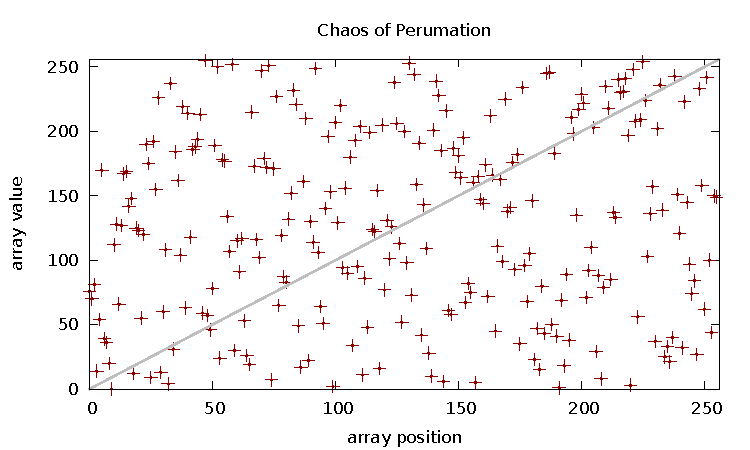
\includegraphics[width=\textwidth]{eclipse/beforerc4.pdf}

\subsubsection{Generieren Sie 100 Schlüsselbytes.}
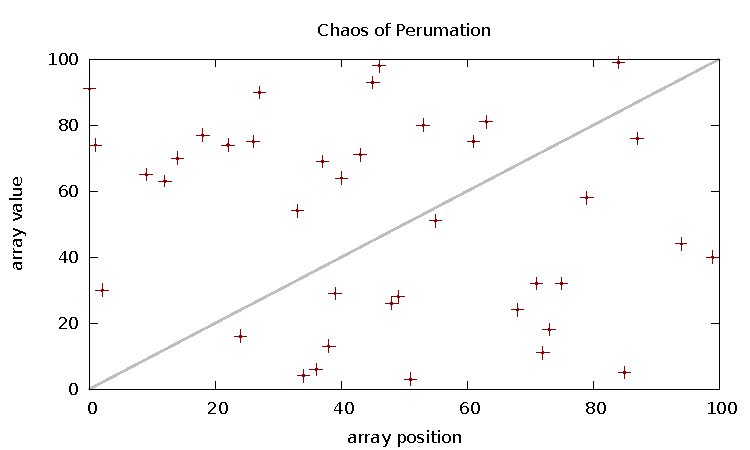
\includegraphics[width=\textwidth]{eclipse/rc4-key-seq.pdf}

\subsubsection{Listen Sie die Permuation $S$ erneut auf.}
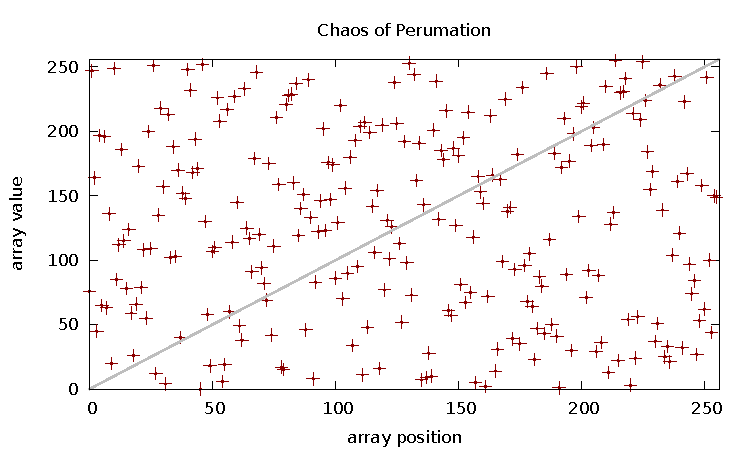
\includegraphics[width=\textwidth]{eclipse/afterrc4.pdf}